\documentclass[12pt, letterpaper, final]{report}
\usepackage{hyperref}
\usepackage{ctable}
\usepackage{graphicx}
\usepackage{amssymb}
\usepackage{amsmath}
\usepackage[section]{placeins}

\author{Devin Schwab (dts34)}
\title{EECS 491 Final Project Report \\ 
\vspace{5 mm}
Learning Basis Functions\\ 
\vspace{5 mm}
 An Evaluation of Protovalue Functions\\
 and the\\
 Representation Policy Iteration Algorithm}

\date{December 12, 2012}

\begin{document}

\maketitle

\section{Abstract}

This project focused on a reinforcement learning technique known as
Representation Policy Iteration (RPI). RPI utilizes samples for a
state space to determine basis functions that are used for
approximation. Traditionally these basis functions have been hand
designed by those creating the reinforcement learning. RPI on the
other hand utilizes information about the state space to create an
approximation. The experiments performed with this framework indicate
that it is indeed a useful algorithm and that while in some cases it may require a
large number of samples to properly converge, when it does converge
the space savings are quite large. All of this experimentation was
done with the intention of understanding the RPI framework so that it
could be used with in conjunction with Bayesian Reinforcement Learning.

\tableofcontents
\newpage
\listoffigures

\section{Background}

\subsection*{Markov Decision Process}

A Markov Decision Process (MDP) is a formal representation of the
problem of making actions in an environment that is not entirely
controlled by the agent. To solve an MDP an agent must determine a
policy that maximizes its expected reward up to some time in the
future.

An MDP is specified by the tuple $(S, A, P_a(s,s'), R_a(s,s'))$ where
S is the set of states in the environment, A is the set of actions the
agent can perform, $P_a(s,s')$ is the transition model and $R_a(s,s')$
specifies the reward model.

MDP's have been a major topic of study for a number of years and so a
number of techniques for solving them have been developed. These
include the model based value iteration algorithm and the model free
Q-learning algorithm. Many of the algorithms are derivatives of these
two algorithms.

Regardless of the technique used to solve the MDP in order for the
solution to be considered optimal it must satisfy the Bellman Optimality
criterion. That is

\[
V^{\pi*} (s) = max_a ( R(s, a) + \gamma \Sigma_{s'} P(s, a, s')
V^{\pi*}(s'))
\]

where $V^{\pi*}$ is the optimal value function and $\gamma$ is the
discount factor. All techniques are trying to solve this criterion
because it is necessary and sufficient for optimality.

The subject
of this project was to examine one such technique known as
Representation Policy Iteration (RPI). And to consider ways in which
it could be incorporated into the Bayesian RL framework.

\subsection*{Q-function Approximation}

In general when using Q-learning or value iteration one generally runs
into the ``curse of dimensionality'' for any reasonable real world
problem. For this reason instead of explicitly tracking $Q^*(s,a)$ for all
states and actions $Q*(s,a)$ is approximated. Often the approximation
is done by hand using heuristics from expert knowledge.

For instance considering the RTS scenario used in the second
programming assignment of this class, that is two armies fighting each
other, some basis functions may be distance to closest enemy, health
of current unit, and health of enemy unit. All of these properties are
computed based on current or previous information.

The Q function can then be approximated by weighting each function and
combining them linearly using the following equation

\[
Q^*(s,a) \approx \hat{Q}^*(s,a) = \Sigma_j \phi_j(s,a)w_j^*
\]

Obviously it would be ideal if these basis functions could be
automatically determined. As in order to come up with good basis
functions one must already have knowledge about the problem domain
that the reinforcement learning agent is trying to solve. The RPI
framework provides a solution to the problem of automatically creating
a set of basis functions for the domain.

One thing to note about the basis function approximation is that it
 can have limited success as the mapping of
the solution onto the basis functions may break the Bellman backup
operator. That is the mapping may no longer be a contraction mapping
and so when using basis functions as an approximation the
reinforcement learning algorithms are no longer guaranteed to converge.

\subsection*{Learning Basis Functions}

The RPI framework utilizes previous work done by Mahadevan {\bf
  CITATION} on Proto-Value Functions (PVFs). Protovalue functions utilize a
lot of the ideas discussed in the field of principle component
analysis. At their basic level proto-value functions are set of
eigenvectors on the representation of some problem's state space.

The PVFs take advantage of the graph operator known as the normalized
graph Laplacian (however, other operators can be
used such as the unnormalized graph Laplacian). The normalized graph
Laplacian is equal to the following $L_n = D^{1/2}LD^{1/2}$ where D is
the degree matrix of the graph and $L=D - A$ where A is the adjacency
matrix. 

By constructing a graph of the state space from a set of
samples, information about the structure of the state space is
represented. The graph laplacian is an operator performed on that
graph that transforms the graph representation into a special matrix
form. This matrix form can be used with eigen vectors and eigen values
to do a form of principal component analysis on the graph. A subset of
these eigen vectors can then be chosen and used as the basis functions.

The eigen vectors of the graph Laplacian form good basis functions for
2 main reasons. The first is that they are orthogonal meaning that
there is no redundancy when the actual value is approximated by being
projected onto these basis functions. Secondly the graph Laplacian
encodes structural information about the space and the eigen vectors
capture key parts of that information.

\subsection*{Least-Squares Policy Iteration}

Least-Squares Policy Iteration (LSPI) is a technique for solving an
MDP by approximating the value function using a set of basis functions
or features. LSPI is an offline algorithm. It converges to a policy
based on a set of sample tuples.

Each sample tuple is of the following form

\[
(s, a, r, s')
\]

Where s is the current state, a is the action taken, r is the reward,
and s' is the resulting state. LSPI uses a set of basis functions and
weights just like discussed earlier. When the basis functions and
weights are represented as matrices the equation for the approximate Q
value becomes

\[
\hat{Q}^*(s,a) = \Phi w^*
\]

In this equation $w^*$ is a column vector of k weights, where k is the
number of basis functions contained within $\Phi$. $\Phi$ is an
$|S||A| \times k$ matrix where $|S|$ is the cardinality of the set of
states and $|A|$ is the cardinality of the set of actions. Each row of
$\Phi$ contains the values of all of the basis functions for a single
(s,a) and each column contains the values of a single basis function
for all (s,a).

The paper that introduces LSPI derives an explict formula that can be
used to solve for the weights. {\bf citation} The formula is the
following

\[ Aw^* = b\]

A and b are approximated using the samples and then the linear
equation is solved explicitly for the weights. This process is
repeated until the policy specified by the weights changes by no more
than $\epsilon$ or the maximum number of iterations is reached.

\subsection*{Representation Policy Iteration (RPI)}

Representation Policy Iteration (RPI) combines the use of PVFs with
the LSPI algorithm to create an offline algorithm that can
approximately solve an MDP.

The basic process is to sample the state space, then construct the
PVFs then run the LSPI algorithm. The RPI framework is what was
experimented with in this project.

\section{Experimental Results}

\subsection*{Comparison of Value Function to Approximation}

\FloatBarrier
\begin{figure}[h!]
\centering

\caption{Comparison of Actual Value Function vs Approximated Value
  Function for Simple 10x10 2 Room problem and 25 PVF}
\label{valueVsQ1}
\end{figure}
\FloatBarrier

\FloatBarrier
\begin{figure}[h!]
\centering
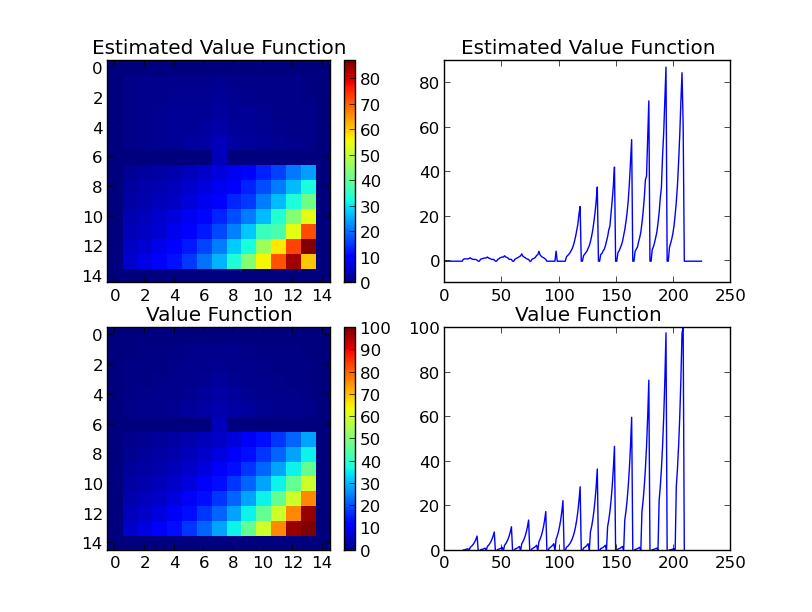
\includegraphics[scale=.5]{images/paper_example_big_V_function_comparison_k75_s5000_graph01.png}
\caption{Comparison of Actual Value Function vs Approximated Value
  Function for Simple 15x15 2 Room problem and 75 PVF}
\label{valueVsQ2}
\end{figure}
\FloatBarrier

\FloatBarrier
\begin{figure}[h!]
\centering

\caption{Comparison of Actual Value Function vs Approximated Value
  Function for Simple 10x10 2 Auto-generated maze problem and 50 PVF}
\label{valueVsQ3}
\end{figure}
\FloatBarrier

\subsection*{Policy Comparison}

While the shape and magnitude of the value function is a very good
approximation the policies vary alot. Graphs of the policy for an
approximated solution are shown next to graphs of the policies for the
actual optimal policy for various numbers of basis functions. The graphs show colors for each state in the
grid. The color key is shown next to the graph.

\FloatBarrier
\begin{figure}[h!]
\centering
\caption{Comparison of Actual Value Function vs Approximated Value
  Function for Simple 10x10 2 Room problem and 25 PVF}
\label{valueVsQ1}
\end{figure}
\FloatBarrier

\FloatBarrier
\begin{figure}[h!]
\centering
\caption{Comparison of Actual Value Function vs Approximated Value
  Function for Simple 15x15 2 Room problem and 75 PVF}
\label{valueVsQ2}
\end{figure}
\FloatBarrier

\FloatBarrier
\begin{figure}[h!]
\centering
\caption{Comparison of Actual Value Function vs Approximated Value
  Function for Simple 10x10 2 Auto-generated maze problem and 50 PVF}
\label{valueVsQ3}
\end{figure}
\FloatBarrier

Its clear that the policies differ in a lot of places. But does this
mean that the policies are useless? In the experiments run these
policies were generally as good as the value function policy. There
are two possible reasons for this.

The first reason is that there are multiple optimal policies. This
is definitely true for the problems examined. For the room problem
domain, so long as the number of
steps taken from the starting position to the goal are the same in two
different policies, those policies are equal in value.

The second reason is that the inoptimality of the approximation is
local. If that local inoptimality is not encountered very often then
on average the approximated policy will appear equal to the optimal
policy.

However, as discussed later in the problems section these local
sections of inoptimal policies can create issues.

\subsection*{Examination of Laplacian Basis Functions}

\FloatBarrier
\begin{figure}[h!]
\centering
\caption{Top 4 Smoothest Normalized Laplacian Basis Functions for
  10x10 2 Room Problem}
\label{laplacianBasis1}
\end{figure}
\FloatBarrier

\FloatBarrier
\begin{figure}[h!]
\centering
\caption{Top 4 Smoothest Normalized Laplacian Basis Functions for
  10x10 3 Room Problem}
\label{laplacianBasis2}
\end{figure}
\FloatBarrier

\FloatBarrier
\begin{figure}[h!]
\centering
\caption{Top 4 Smoothest Normalized Laplacian Basis Functions for
  10x10 Auto-generated maze Problem}
\label{laplacianBasis3}
\end{figure}
\FloatBarrier

\subsection*{Convergence Rate}


The properties of RPI's convergence is still an area that needs to
researched. For this reason I examined the convergence rate for the
rooms problem domain. In all of these experiments
LSPI was set to run till the $|w_{i}-w_{i-1}| \le 10^-5$.

However, it is interesting to examine the convergence rate of the
Q-value approximation to the final value. To examine this the LSPI was
run on the simple 10x10 2 Room problem. The Q-value approximation was
plotted as a 2D color map for 4 different intermediate policy. This
graph is shown in Fig~\ref{Qconvergence1}

\FloatBarrier
\begin{figure}[h!]
\centering
\caption{Approximate Q Value over LSPI Iterations with 25 PVF for
  10x10 2 Room Problem}
\label{Qconvergence1}
\end{figure}
\FloatBarrier

This particular problem converged fairly quickly. The first initial
policy approximation is the only one that is clearly different. The
number of iterations of LSPI that were performed on various problems
was recorded. For each of these problems the world consisted of a
10x10 grid which a number of walls and a single goal worth +100. The
step cost was zero and the actions were up, down, left and right. The
probability of success for each action was .9 and if the action failed
the agent would remain in the same state. Once the goal was reached
the episode was ended and a new one was started.

Using a random policy approximately 5000 samples were collected for
each environment. the RPI algorithm was then run on these samples. In
each of these problems the number of protovalue functions used was 25,
50 and 75. On
average the number of iterations of LSPI until convergence was 9.7

The time to actually compute these representations obviously varies
based on the number of samples, the size of the world, the number of
actions and the number of basis functions. However, the number of
iterations of LSPI that needed to be performed using the basis
functions were quite few. 


\subsection*{Value Function Approximation Efficiency}

To determine how well the RPI framework functions it is important to
have a good understanding of the algorithms efficiency. Efficiency can
mean multiple things, but for this section when I refer to efficiency
I am referring to the following quantity

\[
\eta = \frac{\text{Space Savings}}{\text{Value Function Error}}
\]

The reason this metric is used is because both space savings and the
deviation from the actual value play a large role. For any algorithm
that attempts to calculate the value function, the algorithm is only
useful if the space savings don't cause a large increase in error. 

The bottom term will always remain the same as the value function
error is simply

\[
| V^{*} - \hat{V}^{*}|
\]

The top term, however, depends on the algorithm this method is being
compared to. For instance the space necessary to store all of the
values for Q-learning explicitly is $|S| \times |A|$ for the reward
function, R(s,a), and $|S|^2$ for the Q function, Q(s,a). Where $|S|$ is
the cardinality of the set of states and $|A|$ is the cardinality of
the set of actions.

On the other hand the storage space of the RPI framework algorithm is 
$k|S|+k$ where k is the number of basis functions and $|S|$ is the
cardinality of the set of states.

Therefore for this project the efficiency metric is

\[
\eta = \frac{(|S|^2 + |S||A|) - (k|A| + k)}{|V^{*} - \hat{V}^{*}|}
\]

With this metric if the value function error remains constant as the
space savings increase the efficiency metric will increase and vice
versa. Likewise if the space savings remain constant but the value
function error increases then the efficiency will decrease. 

It is
important to note that while this quantity is called efficiency it is
not a percentage like in the traditional sense. Also this metric will
vary from problem to problem. But it is still useful for comparing
problems in a similar domain.

Using this metric a number of room problems were evaluated with both
value iteration and the the RPI algorithm. The number of PVF's was
determined by when the average steps per episode leveled off. An
example graph is shown in Fig~\ref{performanceComparisonGraph1}

\FloatBarrier
\begin{figure}[h!]
\centering
\caption{Performance Comparison Graph between different PVF's for the
  15x15 2 Room Example}
\label{performanceComparisonGraph1}
\end{figure}
\FloatBarrier

The efficiency metrics for each of the PVFs are as follows

\FloatBarrier
\begin{table}[h!]
  \begin{tabular}{|l|l|l|l|}
  \hline
  {\bf k} & {\bf Space Savings} & {\bf Value Function Error} & $\eta$\\ \hline
  25 & 45875 & 231.19 & 198.43 \\ \hline
  50 & 40225 & 262  & 153.53 \\ \hline
  75 & 34575 &  276.8 & 124.89 \\ \hline
\end{tabular}
\end{table}
\FloatBarrier

As can be seen in the table for this particular experiment 25 basis
functions is the most efficient in terms of reproducing the actual
Value function. As the number of PVF's increased the efficiency
decreased. This is due both to the space savings decreasing as well as
the value function error increasing.

\subsection*{Problems}

While the experiments performed using the RPI framework indicate that
the algorithm does work in general there are a number of problems with
it.

For one the quality of the approximated value function is greatly
affected by the area of the state space that is sampled. If there are
areas of the state space that aren't often visited and if these areas
are missed in the sampling step then the basis functions will be based
off an incorrect interpretation of the state space. As seen in the
laplacian basis functions section the basis functions are strongly
correlated to the spatial properties of the state space. This means
that any missed states can possibly drastically change the
approximated value function.

The solution to this is to sample uniformly over the state space and
to collect a large enough group of samples that with reasonable
confidence one can assume no states were missed.

Another problem is that as shown while the algorithm will converge
relatively quickly the approximation of the value function can be
quite inaccurate. This leads to discrepancies in the policies. As seen
in the policies comparison function while the Value function
approximation may look very similar to the actual Value function the
small discrepancies can lead to widly different policies (although not
necessarily incorrect ones). 

During the experimentation there were
instances when the agent would get stuck in a particular state or in a
loop of states. In general increasing the samples and the number of
basis functions solved these problems. However, it does point out that
whil the approximation of the value function is good, it is not
perfect. And while the policy from the approximated value function may
work for the majority of the states there are still cases where the
policy can fail.

\section{Future Work}

Now that the protovalue basis functions and the RPI have been closely
examined and understood the theory of Bayesian RL can be applied on
top of it. As previously discussed Bayesian RL can be used to solve
the exploration vs exploitation problem. Instead of using Bayesian RL
with Q-learning, the Bayesian RL techniques could be applied to the
RPI framework. This would hopefully allow the learned representations
to be generalized to similar problems in a domain. 

The Bayesian RL could also be used to provide insight into which parts
of a new problem's state space should be sampled first. This would
theoretically reduce the number of samples needed. As the basis
functions and policies would simply need to be repaired when a new
problem from the same domain was encountered.

\section{Conclusion}

Based on the experiments conducted for this project it is clear that
the RPI framework provides real value to the field of reinforcement
learning. Not only does it allow an agent to learn appropriate basis
functions it also drastically cuts down on the amount of information
that must be stored.

While the results can vary based on the state space and actions in
general the algorithm seems to function well while simultaneously
providing tremendous space savings.

\section{References}

\section{Appendix A - Experiment Programs}

A number of experimental programs were created for this project. In
general the programs should be capable of applying to any problem
domain so long as a few functions are implemented for the domain. 

The source code for this project is contained within a Github
repository located at https://github.com/rhololkeolke/eecs\_491\_project

The computer that is running the program requires python, scipy, numpy
and the apgl libraries to function. These can be installed using the
standard python tools such as easy\_install and pip.  The lspiframework directory will also need to be added to the
computer's PYTHONPATH environment variable.

To run the code the basic usage is 

\vspace{5 mm}
{\bf python rooms.py /path/to/map.yaml}
\vspace{5 mm}

where rooms.py is located in the lspi\_examples directory

\section{Appendix B - Bayesian RL}

\subsection*{Bayesian Reinforcement Learning}


\subsection*{Bayesian Exploration}

\subsection*{Bayesian Exploration with RPI}

\end{document}